% !TEX program = xelatex

\documentclass[10pt,a4paper]{article}
\usepackage[top = 1.5cm, bottom = 1.5cm, left = 1.5cm, right = 1.5cm]{geometry}
\usepackage{wrapfig}
\usepackage{float}

\usepackage{titling}
\usepackage[czech]{babel}
\usepackage{graphicx}
\usepackage{lmodern}
\usepackage{hyperref}
\usepackage{setspace}
\usepackage{csvsimple}

\usepackage{amsmath}
\usepackage{amssymb}
\usepackage{gensymb}
\usepackage{mathtools}
\usepackage{units}
\usepackage{bm}
\delimitershortfall=-1pt



% redefine \sqrt
\usepackage{letltxmacro}
\makeatletter
\let\oldr@@t\r@@t
\def\r@@t#1#2{%
\setbox0=\hbox{$\oldr@@t#1{#2\,}$}\dimen0=\ht0
\advance\dimen0-0.2\ht0
\setbox2=\hbox{\vrule height\ht0 depth -\dimen0}%
{\box0\lower0.4pt\box2}}
\LetLtxMacro{\oldsqrt}{\sqrt}
\renewcommand*{\sqrt}[2][\ ]{\oldsqrt[#1]{#2\,}\,}
\makeatother



\DeclarePairedDelimiter\ceil{\lceil}{\rceil}
\DeclarePairedDelimiter\floor{\lfloor}{\rfloor}

\def\ph{\phantom}
\def\vph{\vphantom}
\def\hph{\hphantom}
\def\rzw{\mathrlap}
\def\lzw{\mathllap}
\def\czw{\mathclap}

\def\?{\mathit{?}}

\def\+{+\!\!}
\def\-{-\!\!}

\newcommand{\comm}[2]{\left[ #1, #2 \right]}
\newcommand{\const}[1]{\text{#1}}
\newcommand{\norm}[1]{\left\lVert#1\right\rVert}

\newcommand{\mat}[1]{
    \begin{pmatrix}
        #1
    \end{pmatrix}
}

\newcommand{\mata}[2]{
    \left(
    \begin{array}{@{}#1@{}}
        #2
    \end{array}
    \right)
}

\newcommand{\smat}[2][1]{
    \scalebox{#1}{$\mat{#2}$}
}

\newcommand{\tg}{\operatorname{tg}}
\newcommand{\cotg}{\operatorname{cotg}}
\newcommand{\atg}{\operatorname{atg}}
\newcommand{\cis}{\operatorname{cis}}
\newcommand{\Res}{\operatorname{Res}}
\renewcommand{\Re}{\operatorname{Re}}

\renewcommand{\d}[1]{\;\const{d}#1}
\newcommand{\dd}[2]{\frac{\const{d} #1}{\const{d} #2} \;}
\newcommand{\pd}[2]{\frac{\partial  #1}{\partial  #2} \;}

\newcommand{\bra}[1]{\left< #1 \right|}
\newcommand{\ket}[1]{\left| #1 \right>}
\newcommand{\braket}[2]{\left< #1 \middle| #2 \right>}

\newcommand{\bhat}[1]{\hat{\bm{#1}}}

\newcommand{\e}[1]{\const{e}^{#1}}
\renewcommand{\i}{\const{i}}

\newcommand{\concurrent}{{\upharpoonleft\!\upharpoonright}}
\newcommand{\countercurrent}{{\upharpoonleft\!\downharpoonright}}

\newcommand{\textmath}[2]{\texorpdfstring{$#2$}{#1}}

\begin{document}

\title{Matematika pro Fyziky 2: \\ Doplňující úkol – Fourierova transformace}
\author{Michal Grňo}
\date{\today}

\maketitle

\section{Zadání}
\begin{align*}
    f(x) &= \frac{x^3}{x^4 + 1} \\[5pt]
    \hat{f}(\xi) &= ?
\end{align*}

\section{Řešení}
Funkce $f$ je z $L^2(\mathbb{R})$, proto se její Fourierova transformace rovná tomuto integrálu (ve smyslu rovnosti na $L^2$):
\begin{equation*}
    \hat{f}(\xi)
    = \lim_{R\to\infty} \int_{-R}^{+R} f(x) \; \e{-2\pi\i x\xi} \d{x}
    = \lim_{R\to\infty} \int_{-R}^{+R} \underbrace{\frac{x^3}{x^4 + 1} \; \e{-2\pi\i x\xi}}_{F(x)} \d{x}
\end{equation*}
Budeme tedy integrovat funkci $F(x)$. Přejdeme ke komplexní proměnné a nalezneme singularity integrované funkce.
\begin{align*}
    F(z) &= \frac{z^3}{z^4 + 1} \; \e{-2\pi\i z\xi}
    \\
    \\
    z^4 = -1
    \;&\Leftrightarrow\;
    \e{\i4\phi} = \e{\i(\pi + 2\pi k)} \\
    &\Leftrightarrow\;
    \phi = \frac{\pi}{4} + \frac{\pi}{2} k \\
    &\Leftrightarrow\;
    z \in \{
        \e{\nicefrac{\i\pi}{4}}, \;
        \e{\nicefrac{\i 3\pi}{4}}, \;
        \e{\nicefrac{-\i 3\pi}{4}}, \;
        \e{\nicefrac{-\i\pi}{4}}
    \}
\end{align*}
Integrál vypočteme pomocí integrace podél křivky v komplexní rovině:
\begin{figure}[H]
    \centering
    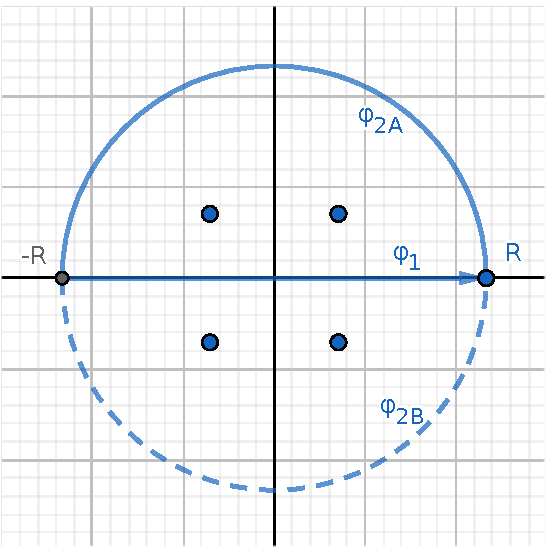
\includegraphics[width=0.3\textwidth]{fourierparam.pdf}
\end{figure}
\begin{gather*}
    \varphi_A = \varphi_1 \oplus \varphi_{2A} \\
    \varphi_B = \varphi_1 \oplus \varphi_{2B}
\end{gather*}
\begin{align*}
    \varphi_{1\ph{A}} &= t \mapsto Rt, \; \ph{^+\i t} t \in [-1, 1] \\
    \varphi_{2A} &= t \mapsto R \e{+\i t}, \; t \in [0, \pi] \\
    \varphi_{2B} &= t \mapsto R \e{-\i t}, \; t \in [0, \pi]
\end{align*}

Provedeme limitní přechod $R\to\infty$. Pro $\xi < 0$ vymizí integrál přes $\varphi_{2A}$, budeme tedy integrovat přes $\varphi_A$. Pro $\xi > 0$ vymizí integrál přes $\varphi_{2B}$, proto budeme integrovat přes $\varphi_B$. Protože se jedná o rovnost na $L^2$, hodnotu pro $\xi=0$ můžeme libovolně doplnit.
\begin{align*}
    \hat{f}(\xi < 0)
    &= \int_{\varphi_1} F(z) \d{z}
    = \int_{\varphi_A} F(z) \d{z}
    = 2\pi\i \left( \Res_{\e{i\pi/4}} F + \Res_{\e{\i 3\pi/4}} F \right),
    \\[10pt]
    \hat{f}(\xi > 0)
    &= \int_{\varphi_1} F(z) \d{z}
    = \int_{\varphi_B} F(z) \d{z}
    = -2\pi\i \left( \Res_{\e{-i\pi/4}} F + \Res_{\e{-\i 3\pi/4}} F \right).
\end{align*}
V přepisu jsme využili reziduové věty. Všechny póly $F$ jsou jednonásobné, proto můžeme rezidua vypočítat následujícím způsobem:
\begin{align*}
    \Res_{\e{\i\pi/4}} F
    &= \lim_{z\to\e{\i\pi/4}} \left( z - \e{\nicefrac{\i\pi}{4}} \right) F(z)
    = \left. \frac{z^3 \e{-2\pi\i z\xi}}{(z-\e{\nicefrac{\i3\pi}{4}})(z-\e{\nicefrac{-\i3\pi}{4}})(z-\e{\nicefrac{-\i\pi}{4}})} \right|_{z=\e{\i\pi/4}}
    \\[5pt]
    &= \left. \frac{z^3 \exp(-2\pi\i\xi|z| \cis \arg z)}{z^3 + z^2 \e{\i\pi/4} - z\e{-\i\pi/2} - \e{-\i\pi/4}} \right|_{z=\e{\i\pi/4}}
    = \frac{
        \e{\nicefrac{3\i\pi}{4}} \; \exp \left(-2\i\pi\xi  (\cos \frac{\pi}{4} + \i \sin \frac{\pi}{4}) \right)
    }{
        (-1+\i)\oldsqrt{2} + \i\e{\nicefrac{\i\pi}{4}} + \e{\nicefrac{3\i\pi}{4}}
    }
    = \frac{1}{4} \, \e{(1-\i)\oldsqrt{2}\pi\xi}
    \\[15pt]
    \Res_{\e{\i3\pi/4}} F
    &= \lim_{z\to\e{\i\pi/4}} \left( z - \e{\nicefrac{\i3\pi}{4}} \right) F(z)
    = \frac{1}{4} \, \e{(1+\i)\oldsqrt{2}\pi\xi}
    \\[15pt]
    \Res_{\e{-\i3\pi/4}} F
    &= \lim_{z\to\e{-\i3\pi/4}} \left( z - \e{\nicefrac{-\i3\pi}{4}} \right) F(z)
    = \frac{1}{4} \, \e{(-1+\i)\oldsqrt{2}\pi\xi}
    \\[15pt]
    \Res_{\e{-\i\pi/4}} F
    &= \lim_{z\to\e{-\i\pi/4}} \left( z - \e{\nicefrac{-\i\pi}{4}} \right) F(z)
    = \frac{1}{4} \, \e{(-1-\i)\oldsqrt{2}\pi\xi}
\end{align*}

\end{document}